\documentclass{article}

\usepackage{fancyhdr}
\usepackage{extramarks}
\usepackage{amsmath}
\usepackage{amsthm}
\usepackage{amsfonts}
\usepackage{tikz}
\usepackage[plain]{algorithm}
\usepackage{algpseudocode}
\usepackage{graphicx}
\usepackage{listings}
\usetikzlibrary{automata,positioning}

%
% Basic Document Settings
%

\topmargin=-0.45in
\evensidemargin=0in
\oddsidemargin=0in
\textwidth=6.5in
\textheight=9.0in
\headsep=0.25in

\linespread{1.1}

\pagestyle{fancy}
\lhead{\hmwkAuthorName}
\chead{\hmwkClass\ (\hmwkClassInstructor\ \hmwkClassTime): \hmwkTitle}
\rhead{\firstxmark}
\lfoot{\lastxmark}
\cfoot{\thepage}

\renewcommand\headrulewidth{0.4pt}
\renewcommand\footrulewidth{0.4pt}

\setlength\parindent{0pt}

%
% Create Problem Sections
%

\newcommand{\enterProblemHeader}[1]{
    \nobreak\extramarks{}{Problem \arabic{#1} continued on next page\ldots}\nobreak{}
    \nobreak\extramarks{Problem \arabic{#1} (continued)}{Problem \arabic{#1} continued on next page\ldots}\nobreak{}
}

\newcommand{\exitProblemHeader}[1]{
    \nobreak\extramarks{Problem \arabic{#1} (continued)}{Problem \arabic{#1} continued on next page\ldots}\nobreak{}
    \stepcounter{#1}
    \nobreak\extramarks{Problem \arabic{#1}}{}\nobreak{}
}

\setcounter{secnumdepth}{0}
\newcounter{partCounter}
\newcounter{homeworkProblemCounter}
\setcounter{homeworkProblemCounter}{1}
\nobreak\extramarks{Problem \arabic{homeworkProblemCounter}}{}\nobreak{}

%
% Homework Problem Environment
%
% This environment takes an optional argument. When given, it will adjust the
% problem counter. This is useful for when the problems given for your
% assignment aren't sequential. See the last 3 problems of this template for an
% example.
%
\newenvironment{homeworkProblem}[1][-1]{
    \ifnum#1>0
        \setcounter{homeworkProblemCounter}{#1}
    \fi
    \section{Problem \arabic{homeworkProblemCounter}}
    \setcounter{partCounter}{1}
    \enterProblemHeader{homeworkProblemCounter}
}{
    \exitProblemHeader{homeworkProblemCounter}
}

%
% Homework Details
%   - Title
%   - Due date
%   - Class
%   - Section/Time
%   - Instructor
%   - Author
%

\newcommand{\hmwkTitle}{Homework\ \#2}
\newcommand{\hmwkDueDate}{October 17, 2016}
\newcommand{\hmwkClass}{STAT 5444}
\newcommand{\hmwkClassTime}{}
\newcommand{\hmwkClassInstructor}{Professor Scott Leman}
\newcommand{\hmwkAuthorName}{Kevin Malhotra}

%
% Title Page
%

\title{
    \vspace{2in}
    \textmd{\textbf{\hmwkClass:\ \hmwkTitle}}\\
    \normalsize\vspace{0.1in}\small{Due\ on\ \hmwkDueDate\ at 3:10pm}\\
    \vspace{0.1in}\large{\textit{\hmwkClassInstructor\ \hmwkClassTime}}
    \vspace{3in}
}

\author{\textbf{\hmwkAuthorName}}
\date{}

\renewcommand{\part}[1]{\textbf{\large Part \Alph{partCounter}}\stepcounter{partCounter}\\}

%
% Various Helper Commands
%

% Useful for algorithms
\newcommand{\alg}[1]{\textsc{\bfseries \footnotesize #1}}

% For derivatives
\newcommand{\deriv}[1]{\frac{\mathrm{d}}{\mathrm{d}x} (#1)}

% For partial derivatives
\newcommand{\pderiv}[2]{\frac{\partial}{\partial #1} (#2)}

% Integral dx
\newcommand{\dx}{\mathrm{d}x}

% Alias for the Solution section header
\newcommand{\solution}{\textbf{\large Solution}}

% Probability commands: Expectation, Variance, Covariance, Bias
\newcommand{\E}{\mathrm{E}}
\newcommand{\Var}{\mathrm{Var}}
\newcommand{\Cov}{\mathrm{Cov}}
\newcommand{\Bias}{\mathrm{Bias}}

\begin{document}

\maketitle

\pagebreak
\begin{homeworkProblem}
N = 30 \\ 
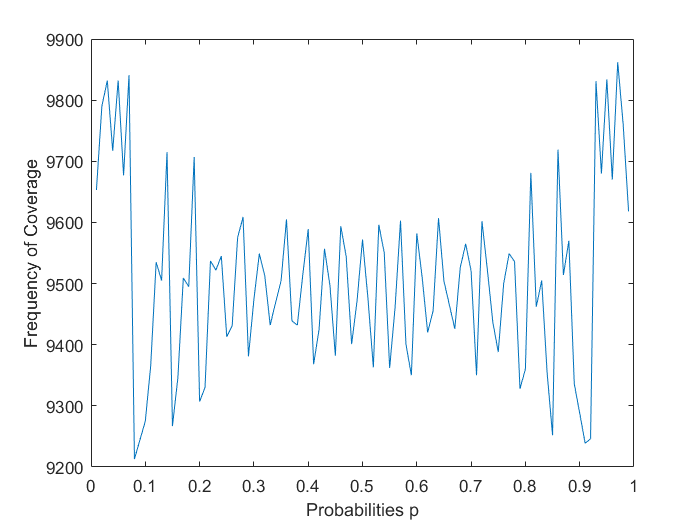
\includegraphics[scale=0.4]{Problem1N30} \\
N = 50 \\
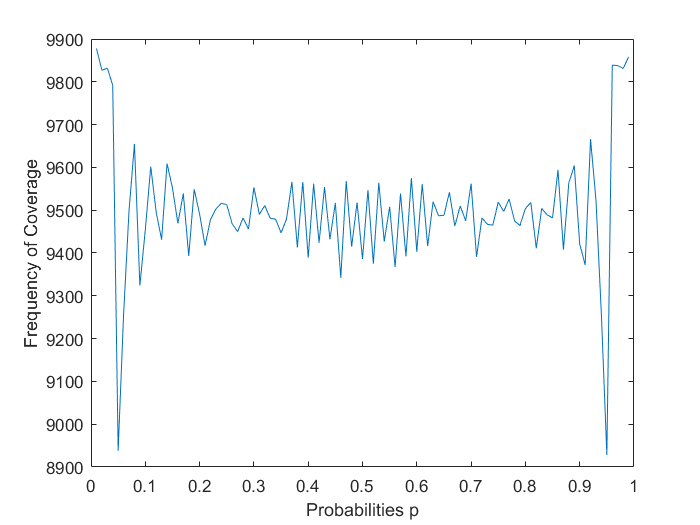
\includegraphics[scale=0.4]{Problem1N50} \\
N = 100 \\
\includegraphics[scale=0.4]{Problem1N100} \\ 
For low probabilities of p  or extremely high probabilities the coverage is within the 95 percent more so
in this example. There is a bit more variance in hitting the 95 percent coverage mark in this Bayesian approach.
The beta prior provides support for the areas with low probability p or high probability p which aids in 
acquiring coverage in those areas. This is particularly useful for ensuring a centered credible interval
for all probabilities p.
\begin{lstlisting}
alpha = 0.5;
beta = 0.5;
frequency = zeros(99, 1);
N = 100;
totalX = zeros(10000, 10000, 1);
temp = 1;
for p=0.01:0.01:0.99
    p
    x = binornd(N, p, 10000, 1);
    alphaStar = x + alpha;
    betaStar = beta + N - x;
    for j=1:10000
        totalX(:, j) = betarnd(alphaStar, betaStar);
    end
    aSort = sort(totalX, 2);
    upper_bound = aSort(:, 9750) >= p;
    lower_bound = aSort(:, 250) <= p;
    frequency(temp, 1) = sum(upper_bound == lower_bound);
    temp = temp + 1;
end
p = 0.01:0.01:0.99;
plot(p, frequency)
xlabel('Probabilities p')
ylabel('Frequency of Coverage')
\end{lstlisting}
\end{homeworkProblem}
%\pagebreak
\begin{homeworkProblem}
\begin{align*} 
p(\phi | X) &= \int_{}^{} p(\mu | X \phi) p(\phi) p(\mu) d\mu \\ 
p(\phi | X) &= \int_{}^{} \prod_{i=1}^N \frac{\phi^2}{\sqrt{2\pi}} 
	e^{\frac{\phi}{2}(x-\mu)^2} d\mu \\
p(\phi | X) &\propto \phi^{\frac{N}{2}-1} \int_{}^{} 
	e^{\frac{\phi}{2}(x-\mu)^2} d\mu \\
p(\phi | X) &\propto \phi^{\frac{N}{2}-1} \int_{}^{} 
	e^{\frac{\phi}{2}((\sum_{i=1}^{N}x_i^2) - 2\mu \sum_{i=1}^{N}x_i  + N\mu^2)} d\mu \\
p(\phi | X) &\propto \phi^{\frac{N}{2}-1}e^{\frac{-\phi}{2}(\sum_{i=0}^{N} x^2)} \int_{}^{}     
	e^{\frac{\phi}{2}(N\mu^2 - 2\mu \sum_{i=1}^{N}x_i)} d\mu \\
\end{align*}
To acquire the pdf we must have this \\
\begin{align*}
V &= (\phi N)^{-1} = \frac{\phi^{-1}}{N} \\ 
E &= \frac{\phi^{-1}}{N} * \sum_{i=1}^N x_i \phi = \bar{x} \\
pdfNormal &=\int_{}^{} e^{\frac{-1}{2V}(u^2 - 2\bar{x} \mu + \bar{x}^2)} \\ 
\end{align*}
Thus, we integrate to 1
\begin{align*}
p(\phi | X) &\propto \phi^{\frac{N}{2}-1}e^{\frac{-\phi}{2}(\sum_{i=0}^{N} x^2)} \int_{}^{}     
	e^{\frac{\phi}{2}(N\mu^2 - 2\mu \sum_{i=1}^{N}x_i)} d\mu *
	\frac{\frac{1}{\sqrt{2\pi V} e^{\frac{-1}{2} \frac{\bar{x}^2}{V}}}}
	{\frac{1}{\sqrt{2\pi V} e^{\frac{-1}{2} \frac{\bar{x}^2}{V}}}}\\
p(\phi | X) &\propto \phi^{\frac{N}{2}-1}e^{\frac{-\phi}{2}(\sum_{i=0}^{N} x^2)}
	\sqrt{2\pi V} e^{\frac{1}{2} \frac{\bar{x}^2}{V}}\\
p(\phi | X) &\propto \phi^{\frac{N}{2}-1}e^{\frac{-\phi}{2}(\sum_{i=0}^{N} x^2)}
	\sqrt{2\pi \frac{\phi^{-1}}{N}} e^{\frac{1}{2} \frac{\bar{x}^2}{\frac{\phi^{-1}}{N}}}\\
p(\phi | X) &\propto \phi^{\frac{N}{2}-1}e^{\frac{-\phi}{2}(\sum_{i=0}^{N} x^2)}
	\phi^\frac{-1}{2} e^{\frac{1}{2} N\bar{x}^2 \phi }\\
p(\phi | X) &\propto \phi^{\frac{N-1}{2}-1}e^{\frac{-\phi}{2}(\sum_{i=0}^{N} x^2)}
	 e^{\frac{-1}{2}(- N\bar{x}^2 \phi) }\\
p(\phi | X) &\propto \phi^{\frac{N-1}{2}-1}e^{\frac{-\phi}{2}(\sum_{i=0}^{N} x^2 -N\bar{x}^2)}\\
p(\phi | X) &\propto \phi^{\frac{N-1}{2}-1}
	e^{\frac{-\phi}{2}(\sum_{i=0}^{N} x^2 -\sum_{i=0}^{N}\bar{x}^2)}\\
\end{align*}
The follow theorem is used:
\begin{align*}
E(x-\bar{x})^2) &= E(x^2 -2x\bar{x} + \bar{x}^2) \\
     				 &= E(x^2 - 2E(x)^2 + E(x)^2) \\
     				 &= E(x^2) - E(x)^2 \\
N* E(x-\bar{x})^2 &= \sum_{i=0}^N (x-\bar{x})^2 \\
N*E(x^2) - N*E(x)^2 &= (\sum_{i=0}^{N} x^2 -\sum_{i=0}^{N}\bar{x}^2) \\
\end{align*}
Thus, we can do the following
\begin{align*}
p(\phi | X) &\propto \phi^{\frac{N-1}{2}-1}
	e^{\frac{-\phi}{2}(\sum_{i=0}^{N} x^2 -\sum_{i=0}^{N}\bar{x}^2)}\\
p(\phi | X) &\propto \phi^{\frac{N-1}{2}-1}
	e^{\frac{-\phi}{2}(\sum_{i=0}^N (x-\bar{x})^2)}\\
s^2 &= \frac{\sum(x_i - \bar{x})^2}{N-1} \\ 
p(\phi | X) &\propto \phi^{\frac{N-1}{2}-1}
	e^{\frac{-\phi}{2}(s^2(N-1))} \\
p(\phi | X) &- Gamma\big[\frac{N-1}{2}, \frac{(s^2(N-1))}{2}\big] \\
\end{align*}
Part 2: \\ 
\begin{align*}
P(\widetilde{x}|X) &= \int P(\widetilde{x}|X\phi)P(\phi)d\phi \\
P(\widetilde{x}|X) &= \int_{}^{} \frac{\phi^{\frac{1}{2}}}{\sqrt{2\pi}(1+\frac{1}{N})}
	e^{\frac{-\phi}{2} \frac{(\widetilde{x} - \bar{x})^2}{(1+\frac{1}{N})}} 
	\phi^{\frac{N-1}{2}-1} e^{\frac{-\phi}{2}(s^2(N-1))} \\
P(\widetilde{x}|X) &\propto \int_{}^{} \phi^{\frac{N}{2} -1}
	e^{\frac{-\phi}{2} \frac{(\widetilde{x} - \bar{x})^2}{(1+\frac{1}{N})}}
     e^{\frac{-\phi}{2}(s^2(N-1))}	\\
P(\widetilde{x}|X) &\propto \int_{}^{} \phi^{\frac{N}{2} -1}
	e^{\frac{-\phi}{2}(\frac{(\widetilde{x} - \bar{x})^2}{(1+\frac{1}{N})} + (s^2(N-1)))} \\
P(\widetilde{x}|X) &\propto \int_{}^{} \phi^{\frac{N}{2} -1} 
	e^{\frac{-\phi}{2}(\frac{(\widetilde{x} - \bar{x})^2}{(1+\frac{1}{N})} + (s^2(N-1)))} *
	\frac{\frac{\Gamma(N/2)}{\Bigg[\frac{1}{2}*(\frac{(\widetilde{x} - \bar{x})^2}{(1+\frac{1}{N})} + (s^2(N-1)))\Bigg]^{N/2}}}{\frac{\Gamma(N/2)}{\Bigg[\frac{1}{2}*(\frac{(\widetilde{x} - \bar{x})^2}{(1+\frac{1}{N})} + (s^2(N-1)))\Bigg]^{N/2}}} \\
P(\widetilde{x}|X) &\propto \frac{\Gamma(N/2)}{\Bigg[\frac{1}{2}*(\frac{(\widetilde{x} - \bar{x})^2}
	{(1+\frac{1}{N})} + (s^2(N-1)))\Bigg]^{N/2}} \\
P(\widetilde{x}|X) &\propto \Bigg[\frac{(\widetilde{x} - \bar{x})^2}
	{(1+\frac{1}{N})} + (s^2(N-1))\Bigg]^{-N/2} \\
\end{align*}
\begin{align*}
P(\widetilde{x}|X) &\propto \Bigg[\frac{(\widetilde{x} - \bar{x})^2}
	{(1+\frac{1}{N})} + (s^2(N-1))\Bigg]^{-N/2} \\
P(\widetilde{x}|X) &\propto \Bigg[1 + \frac{(\widetilde{x} - \bar{x})^2}
	{(1+\frac{1}{N})(s^2(N-1))} \Bigg]^{-N/2} \\
P(\widetilde{x}|X) &\propto \Bigg[1 + \frac{(\widetilde{x} - \bar{x})^2}
	{(1+\frac{1}{N})(s^2(N-1))} \Bigg]^{\frac{-(N-1)+1}{2}} \\
\widetilde{x}|X &- t(\bar{x}, s^2(1+\frac{1}{N}, N -1)
\end{align*}
\end{homeworkProblem}
\pagebreak
\begin{homeworkProblem}
\begin{align*}
p(x|\mu, \sigma^2, \gamma) &\propto (\phi/\gamma)^{1/2}exp(-\frac{\phi}{2}\frac{(x-\mu)^2}{\gamma} \\
p(\phi) &\propto \phi^{\alpha -1}e^{-\beta\phi}\\
p(x|\mu, \gamma) &\propto \int p(x|\mu, \sigma^2, \gamma) p(\phi) d\phi \\
p(x|\mu, \gamma) &\propto \int \frac{\phi^{\frac{1}{2}}}{\gamma}
	e^{\bigg[ \frac{-\phi}{2}\frac{(x-\mu)^2}{\gamma}\bigg]} * \phi^{\alpha -1}e^{-\beta\phi} \\
p(x|\mu, \gamma) &\propto \int \frac{\phi^{\frac{1}{2}+\alpha-1}}{\gamma}
	e^{\bigg[ \frac{-\phi}{2}\frac{(x-\mu)^2}{\gamma} -\beta\phi \bigg]}  \\	
p(x|\mu, \gamma) &\propto \int \frac{\phi^{\frac{1}{2}+\alpha-1}}{\gamma}
	e^{-\phi \bigg[\frac{(x-\mu)^2}{2\gamma} +\beta \bigg]}  \\	
p(x|\mu, \gamma) &\propto \int \frac{\phi^{\frac{1}{2}+\alpha-1}}{\gamma}
	e^{-\phi \bigg[\frac{(x-\mu)^2}{2\gamma} +\beta \bigg]} * 
	\frac{\frac{\Gamma(\frac{1}{2}+\alpha)}{\bigg[\frac{(x-\mu)^2}{2\gamma} +\beta \bigg]^{\frac{1}{2}+\alpha}}}
	{\frac{\Gamma(\frac{1}{2}+\alpha)}{\bigg[\frac{(x-\mu)^2}{2\gamma} +\beta \bigg]^{\frac{1}{2}+\alpha}}}\\	
p(x|\mu, \gamma) &\propto 
	\frac{\Gamma(\frac{1}{2}+\alpha)}{\bigg[\frac{(x-\mu)^2}{2\gamma} +\beta \bigg]
	^{\frac{1}{2}+\alpha}}\\
p(x|\mu, \gamma) &\propto 
	\frac{1}{\bigg[\frac{(x-\mu)^2}{2\gamma} + \beta \bigg]^{\frac{1}{2}+\alpha}} \\ 
p(x|\mu, \gamma) &\propto 
	\frac{1}{\bigg[\frac{(x-\mu)^2}{2\gamma} + 1 \bigg]^{\frac{1}{2}+\frac{1}{2}}},
	 \alpha = \frac{1}{2}, \beta = 1 \\
\end{align*}
Part 3: \\ 
\( \mu = 0, \gamma = 0.5, min = -4.18, max = 3.1\) \\
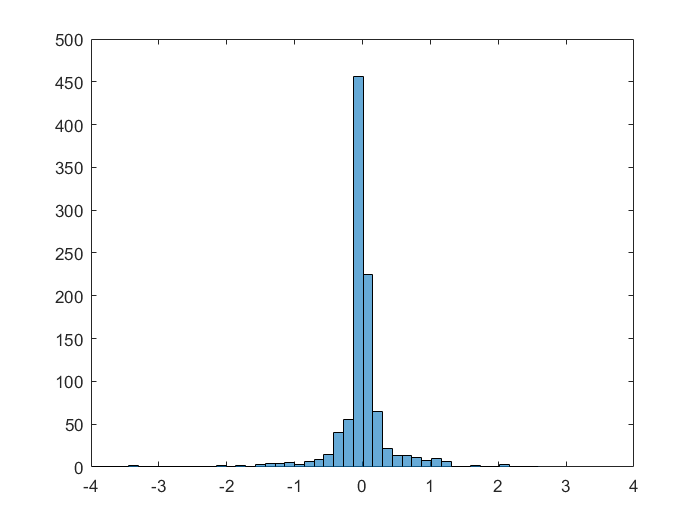
\includegraphics[scale=0.4]{cauchy1} \\
\( \mu = 0, \gamma = 1, min = -9.74, max = 7.094\) \\
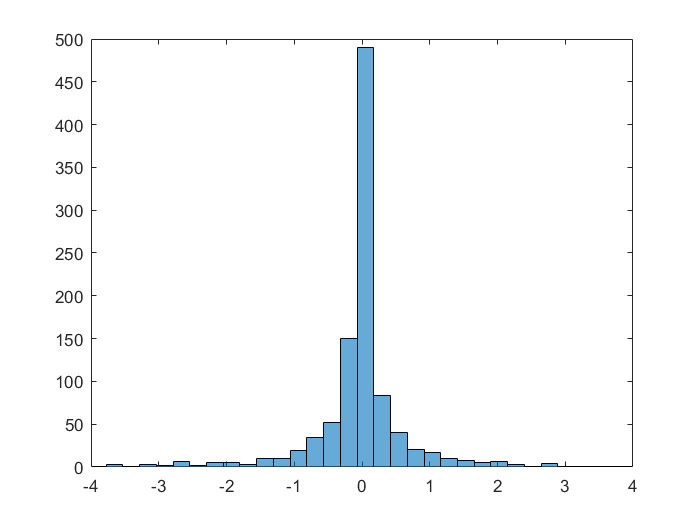
\includegraphics[scale=0.4]{cauchy2} \\
\( \mu = 0, \gamma = 2, min = -18.51, max = 11.33\) \\
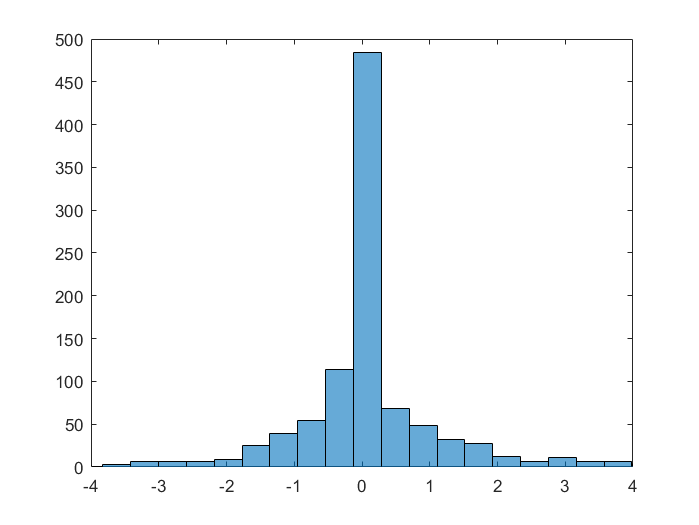
\includegraphics[scale=0.4]{cauchy3} \\
\( \mu = -2, \gamma = 1, min = -6.18, max = 6.51\) \\
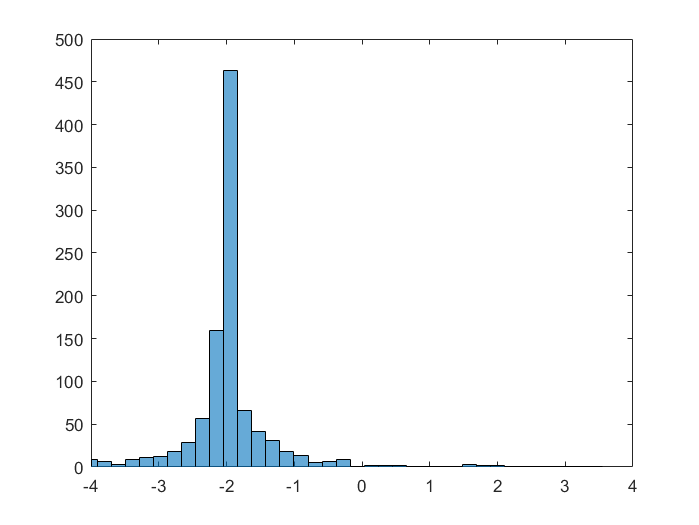
\includegraphics[scale=0.4]{cauchy4}
\begin{lstlisting}
mu = 0;
gamma = 0.5;
post = normrnd(mu, sigma*gamma);
figure(1), histogram(post, 50)
axis([-4 4 0 500])
min(post)
max(post)
\end{lstlisting}
\end{homeworkProblem}
\begin{homeworkProblem}
MAP is not invariant to transformations. Using a normal distributed MAP estimator with no prior the MAP estimator is the value 0. Applying a transformation of \(\tau(\theta) = \theta^2\) will result in the MAP estimator being the value 0.7. When we apply the transformation to the original value 0 it will not yield the value 0.7. Thus, the MAP is not invariant to transformations.
\end{homeworkProblem}
%\pagebreak
\begin{homeworkProblem}
Part 1: \\ 
In previous derivations we have the following posterior: \( \mu - N(\bar{x}, \frac{\sigma^2}{N}) \) \\
To determine if the predictive distribution is normal we can apply the prediction distribution function.
Since it ends being an integral of a normal * normal it will end up being a normal just be rules of
conjugate priors. Proof Below \\ \\
\begin{align*}
P(\widetilde{x}|X, \sigma^2) &= \int \frac{1}{\sqrt{2\pi}\sigma} * 
	e^{\frac{-1}{2}\frac{(\widetilde{x}-\mu)^2}{\sigma^2}} *
	\frac{1}{\sqrt{2\pi}\frac{\sigma}{\sqrt{N}}} *
	e^{\frac{-1}{2}\frac{(\mu - \bar{x})^2}{\frac{\sigma^2}{N}}} d\mu \\
P(\widetilde{x}|X, \sigma^2) &\propto \int  
	e^{\frac{-1}{2}\frac{(\widetilde{x}-\mu)^2}{\sigma^2}} *
	e^{\frac{-1}{2}\frac{(\mu - \bar{x})^2}{\frac{\sigma^2}{N}}} d\mu \\
P(\widetilde{x}|X, \sigma^2) &\propto \int  
	e^{\frac{-1}{2}\frac{\widetilde{x}^2 -2\widetilde{x}\mu + \mu^2}{\sigma^2}} *
	e^{\frac{-1}{2}\frac{\mu^2 -2\mu \bar{x} + \bar{x}^2}{\frac{\sigma^2}{N}}} d\mu \\
P(\widetilde{x}|X, \sigma^2) &\propto e^{\frac{-1}{2}\frac{\widetilde{x}^2}{\sigma^2}} \int  
	e^{\frac{-1}{2}{(\mu^2\bigg[ \frac{1}{\sigma^2}+\frac{N}{\sigma^2}\bigg] 
	- 2\mu\bigg[\frac{\bar{x}N}{\sigma^2} + \frac{\widetilde{x}}{\sigma^2} \bigg])}} d\mu \\
V* &= (\frac{N+1}{\sigma^2})^{-1} = \frac{\sigma^2}{N+1} \\
E* &= \bigg[\frac{\bar{x}N}{\sigma^2} + \frac{\widetilde{x}}{\sigma^2} \bigg] \frac{\sigma^2}{N+1} 
	= \frac{\widetilde{x} + \bar{x}N}{N+1}\\
Normal Dist &= \int e^{\frac{-1}{2} \frac{(\mu - \E*)^2}{V*}} \\
P(\widetilde{x}|X, \sigma^2) &\propto e^{\frac{-1}{2}\frac{\widetilde{x}^2}{\sigma^2}}
	e^{\frac{1}{2}(\frac{\widetilde{x} + \bar{x}}{N+1})^2 (\frac{N+1}{\sigma^2})} d\mu \\
P(\widetilde{x}|X, \sigma^2) &\propto e^{\frac{-1}{2}\frac{\widetilde{x}^2}{\sigma^2})}
	e^{\frac{1}{2}(\frac{\widetilde{x}^2 + 2\widetilde{x}\bar{x}N + (\bar{x}N)^2}{N+1})^2 
	(\frac{N+1}{\sigma^2})} d\mu \\
P(\widetilde{x}|X, \sigma^2) &\propto e^{\frac{-1}{2}(\widetilde{x}^2
	\bigg[\frac{1}{\sigma^2} - \frac{1}{(N+1)\sigma^2}\bigg] - 2\widetilde{x}
	\bigg[\frac{\bar{x}N}{(N+1)^2} * \frac{N+1}{\sigma^2}\bigg])} d\mu \\
\end{align*}
Thus, we can see that the following intermediate steps above is in fact normally distributed.
This formalizes to the posterior provided in the problem. \\
Part 2: \\
\begin{align*}
E[\widetilde{x}|X \sigma^2] &= E[E[\widetilde{x}|\mu X \sigma^2]] | X \sigma^2] \\
E[\widetilde{x}|X \sigma^2] &= E(\mu | X \sigma^2) = \bar{x} \\
V[\widetilde{x}|X \sigma^2] &= V[E[\widetilde{x}|\mu X \sigma^2] | X \sigma^2] + 
	E[V[\widetilde{x}|\mu X \sigma^2]|X \sigma^2]
V[\widetilde{x}|X \sigma^2] &= V[\mu | X \sigma^2) + E(\sigma^2 | X \sigma^2) = 
	\frac{\sigma^2}{N} + \sigma^2
\end{align*}
\end{homeworkProblem}
\end{document}